\section{Threshold and search of contours}
To measure a object bypassing the camera field the outlines of the object are needed. The challenge here is to find the edges of an object with little computing power in such a short time that the measurement time does not become useless. For further processing the edges have to be represented by an one pixel thick line. This section shows the used method and implementation of the further used edge detection. The ISP driver of the Jetson Nano is used in the automatic mode. In this configuration the ISP tries to keep the mean of the image close to the value 128, which resembles the middle of its range. Since the gStreamer pipeline handling over Python is somewhat complicated, the camera is only used in automatic mode.

\subsection{Threshold}
To determine a good threshold method a short look at the histogram is the first step to success.  
\begin{figure}[ht]
	\subfigure[\label{development:thre1}]{\fbox{\includegraphics[width=0.5\linewidth, height=5cm]{3-development/threshold/saved5.png}}}
	\subfigure[\label{development:thre2}]{\fbox{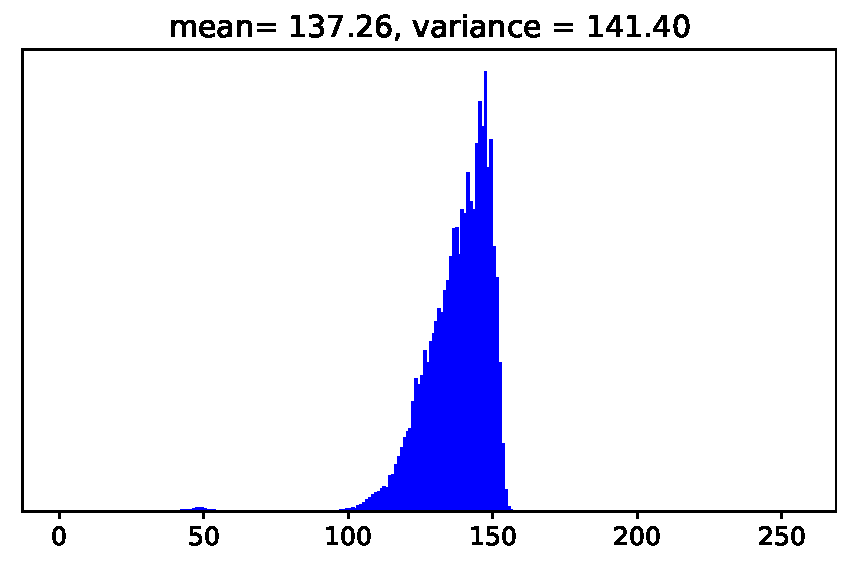
\includegraphics[width=0.5\linewidth, height=5cm]{3-development/threshold/hist_pattern2.pdf}}}
	\subfigure[\label{development:thre3}]{\fbox{\includegraphics[width=0.5\linewidth, height=5cm]{3-development/threshold/saved2.png}}}
	\subfigure[\label{development:thre4}]{\fbox{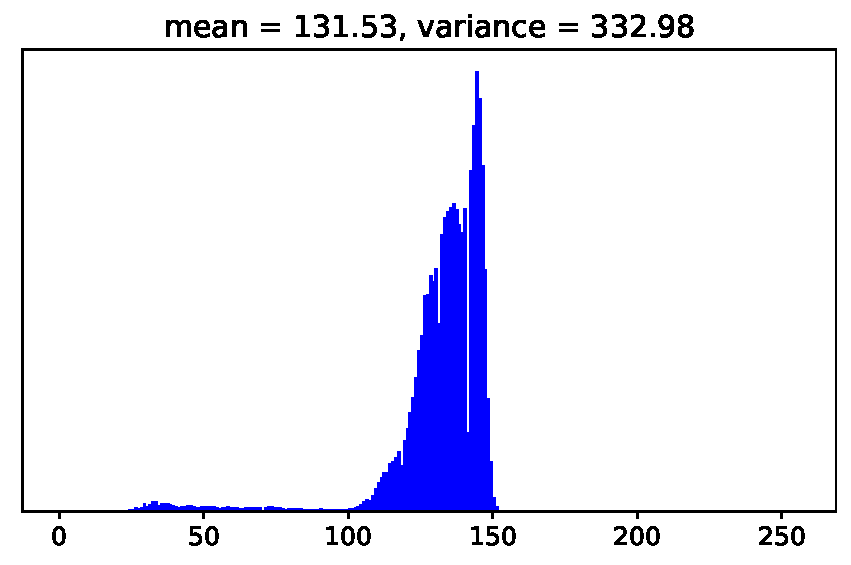
\includegraphics[width=0.5\linewidth, height=5cm]{3-development/threshold/hist_feder2.pdf}}}
\end{figure}
In the picture \ref{development:thre1} the back light is running and the calibration pattern is in place but no object to measure. The corresponding histogram \ref{development:thre2} shows 